\section{Proposed Work}
\large
This report proposes an analysis of different types of Merkle tree’s and choosing the best one for data integrity auditing scheme based on a Merkle hash tree and blockchain, aiming to improve the efficiency and security of data storage. The scheme uses blockchain instead of a third-party auditor to ensure reliability and prevent data tampering. We are going to analyze the time complexity and space complexity of different types of Merkle Tree’s. Among SMT, Quad Merkle tree and Hybrid Merkle tree We are going to choose the efficient one based on time complexity analysis.

1) In the proposed work, we design a blockchain-based auditing scheme that uses blockchain instead of a third-party auditor to ensure the reliability of data auditing. It also makes the data stored in the cloud more secure and private and prevents data from being tampered with by people with ulterior motives.

2) Our scheme is based on the sparse Merkle hash tree scheme. The sparse Merkle hash tree is more efficient than the general binary Merkle hash tree, using the root of the Merkle hash tree to verify the integrity of the data, which greatly improves computing and storage efficiency.

3) In this paper, several smart contracts are deployed, and automatic verification of auditing activities is achieved using the deployment of smart contracts on the blockchain, allowing us to grasp the integrity of the data more easily.

4) Safety analysis and performance evaluation of the proposed scheme proved its feasibility of the scheme.

\subsection{Data Model of Proposed Work}
The system model of a blockchain based cloud storage auditing scheme involves three entities, which are client, cloud, and blockchain.

1)\textbf{ Client:} The client refers to the data owner, which can be an individual or an organization. The client has a large amount of data and needs to use the cloud server to store the data and reduce its own storage and computing burden.

2) \textbf{Blockchain: }The blockchain stores the root of the Merkle hash tree constructed from the client's data and is used to verify the integrity of the data.After encrypting the data, the client generates a quad Merkle hash tree using the data block signatures, sends the root Root to the blockchain for storage, and sends the encrypted data along with the Merkle hash tree to the cloud for storage but loses control of the data. 
Therefore, a query message is sent to the cloud and the blockchain, and the cloudreturns the verification information related to the query to the blockchain. The blockchain uses the information sent by the cloud to calculate the new Merkle hash tree root Root´, compare it with the original root Root, verify its integrity, and send the result to the client.

3) \textbf{Cloud:} The cloud server is managed and maintained by the cloud service provider with massive storage space and computing resources, which lays the foundation for storing large amounts of data from the client and verifying the integrity of the stored data.


\subsection{Initialization Phase}

First, the client generates a random value \textit{sk ∈ Zp} as its 
private key and computes the public key \textit{pk}, and sends the 
relevant key information for verifying the signature to the 
blockchain. 
Second, the client first encrypts the data file and then splits 
the encrypted data file F into n blocks, i.e., \textit{F = {m1, m2, ..., 
mn}}.
Third, the data tag Tagi of each block mi is computed with 
the private key, and the signature method we use here is the 
ZSS short signature method. The set of tags of data file F is T
=\textit{{Tag1, Tag2, ..., Tagi}}.
Fourth, the client generates a quad Merkle hash tree with 
data tags and sends the root Root of the tree to the blockchain 
for storage
Finally, the client outsources the encrypted data file F and 
the quad Merkle hash tree to the cloud, and the client deletes 
the local data file and tags. The cloud will check the integrity 
of the data block before accepting the outsourced data to 
prevent malicious clients. The checking process is like the 
verification phase described below.
The process of the initialization phase is shown in Figure.

\begin{figure}[H]
    \centering
    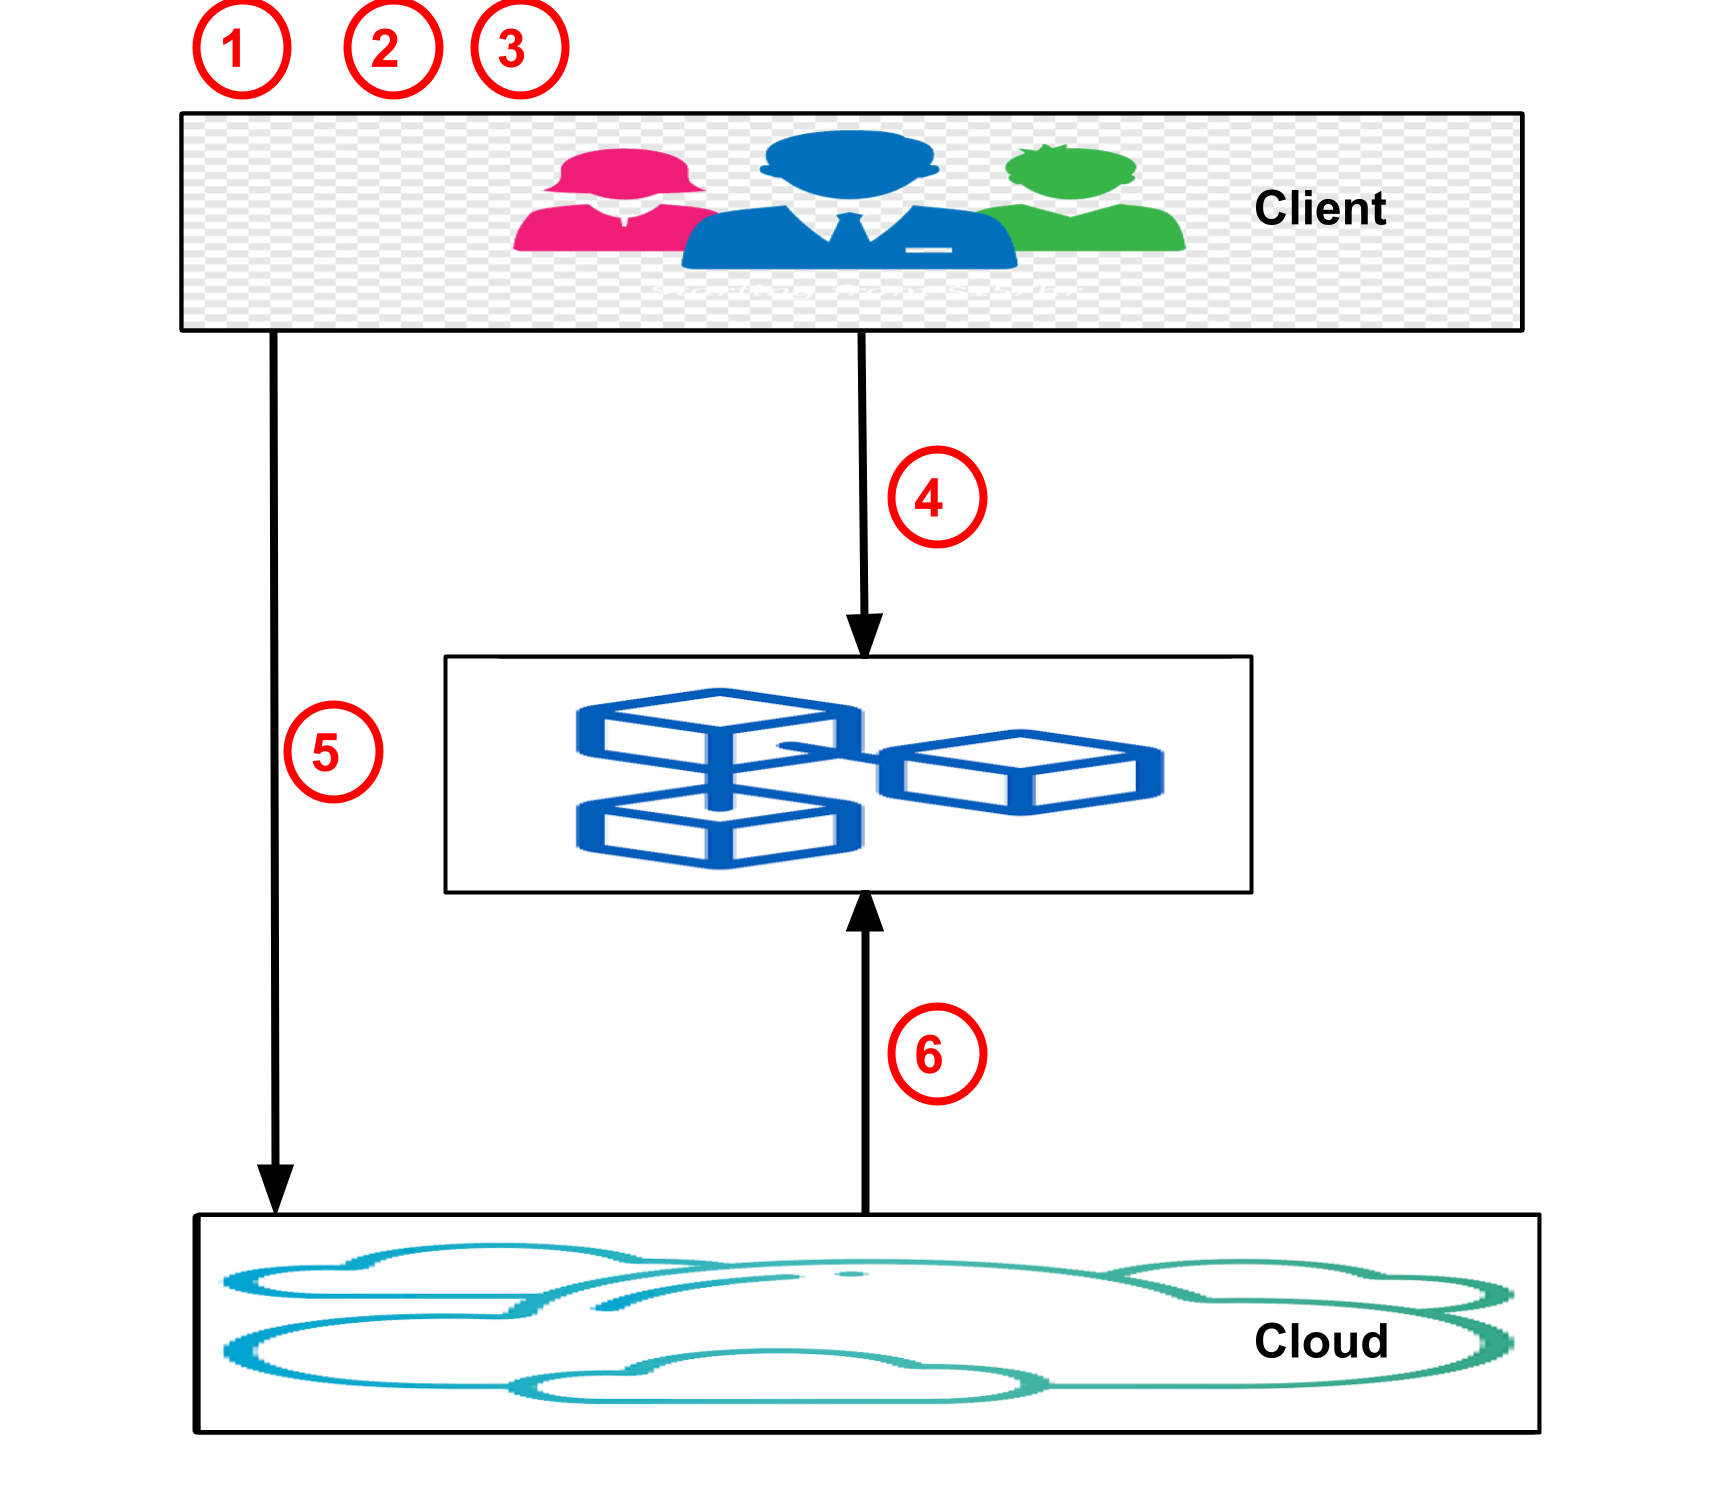
\includegraphics[scale=0.2]{figures/Untitled drawing (3).png}
    \caption{The process of initialization phase}
 
\end{figure}

1) Calculate the public-private key.

2) Slice the data file.

3) Calculate the data tags and generate the Merkle hash tree.

4) Send key-related information and Merkle hash tree root.

5) Encrypted data files and Merkle hash trees.

6) Verify data file integrity.

\subsection{Verification Phase}

First, the client, as a verifier, randomly selects b elements to 
form the query index set \textit{I = {v1, v2, ...vb}}, b belongs to range \textit{[1, n]}, and forms the audit query chal, and sends it to the cloud.
Second, the cloud receives the query message chal and 
sends the corresponding series of encrypted data blocks mi, 
data block signatures Tagi, and random queries vi and auxiliary 
information σ to the blockchain.
Third, the blockchain verifies the correctness of the 
signatures using the key information sent by the client, and 
after successful verification, Root' is calculated using the smart 
contract deployed on the blockchain based on the signatures 
Tagi and the random queries vi and the auxiliary information σ, 
where \textit{v1 ≤ i ≤ vb}.
Finally, the blockchain compares Root and Root' by the 
verifyContract. if Root = Root', the data is complete, otherwise,
the stored data is corrupted, and the verification result is 
returned to the client.

\begin{figure}[H]
    \centering
    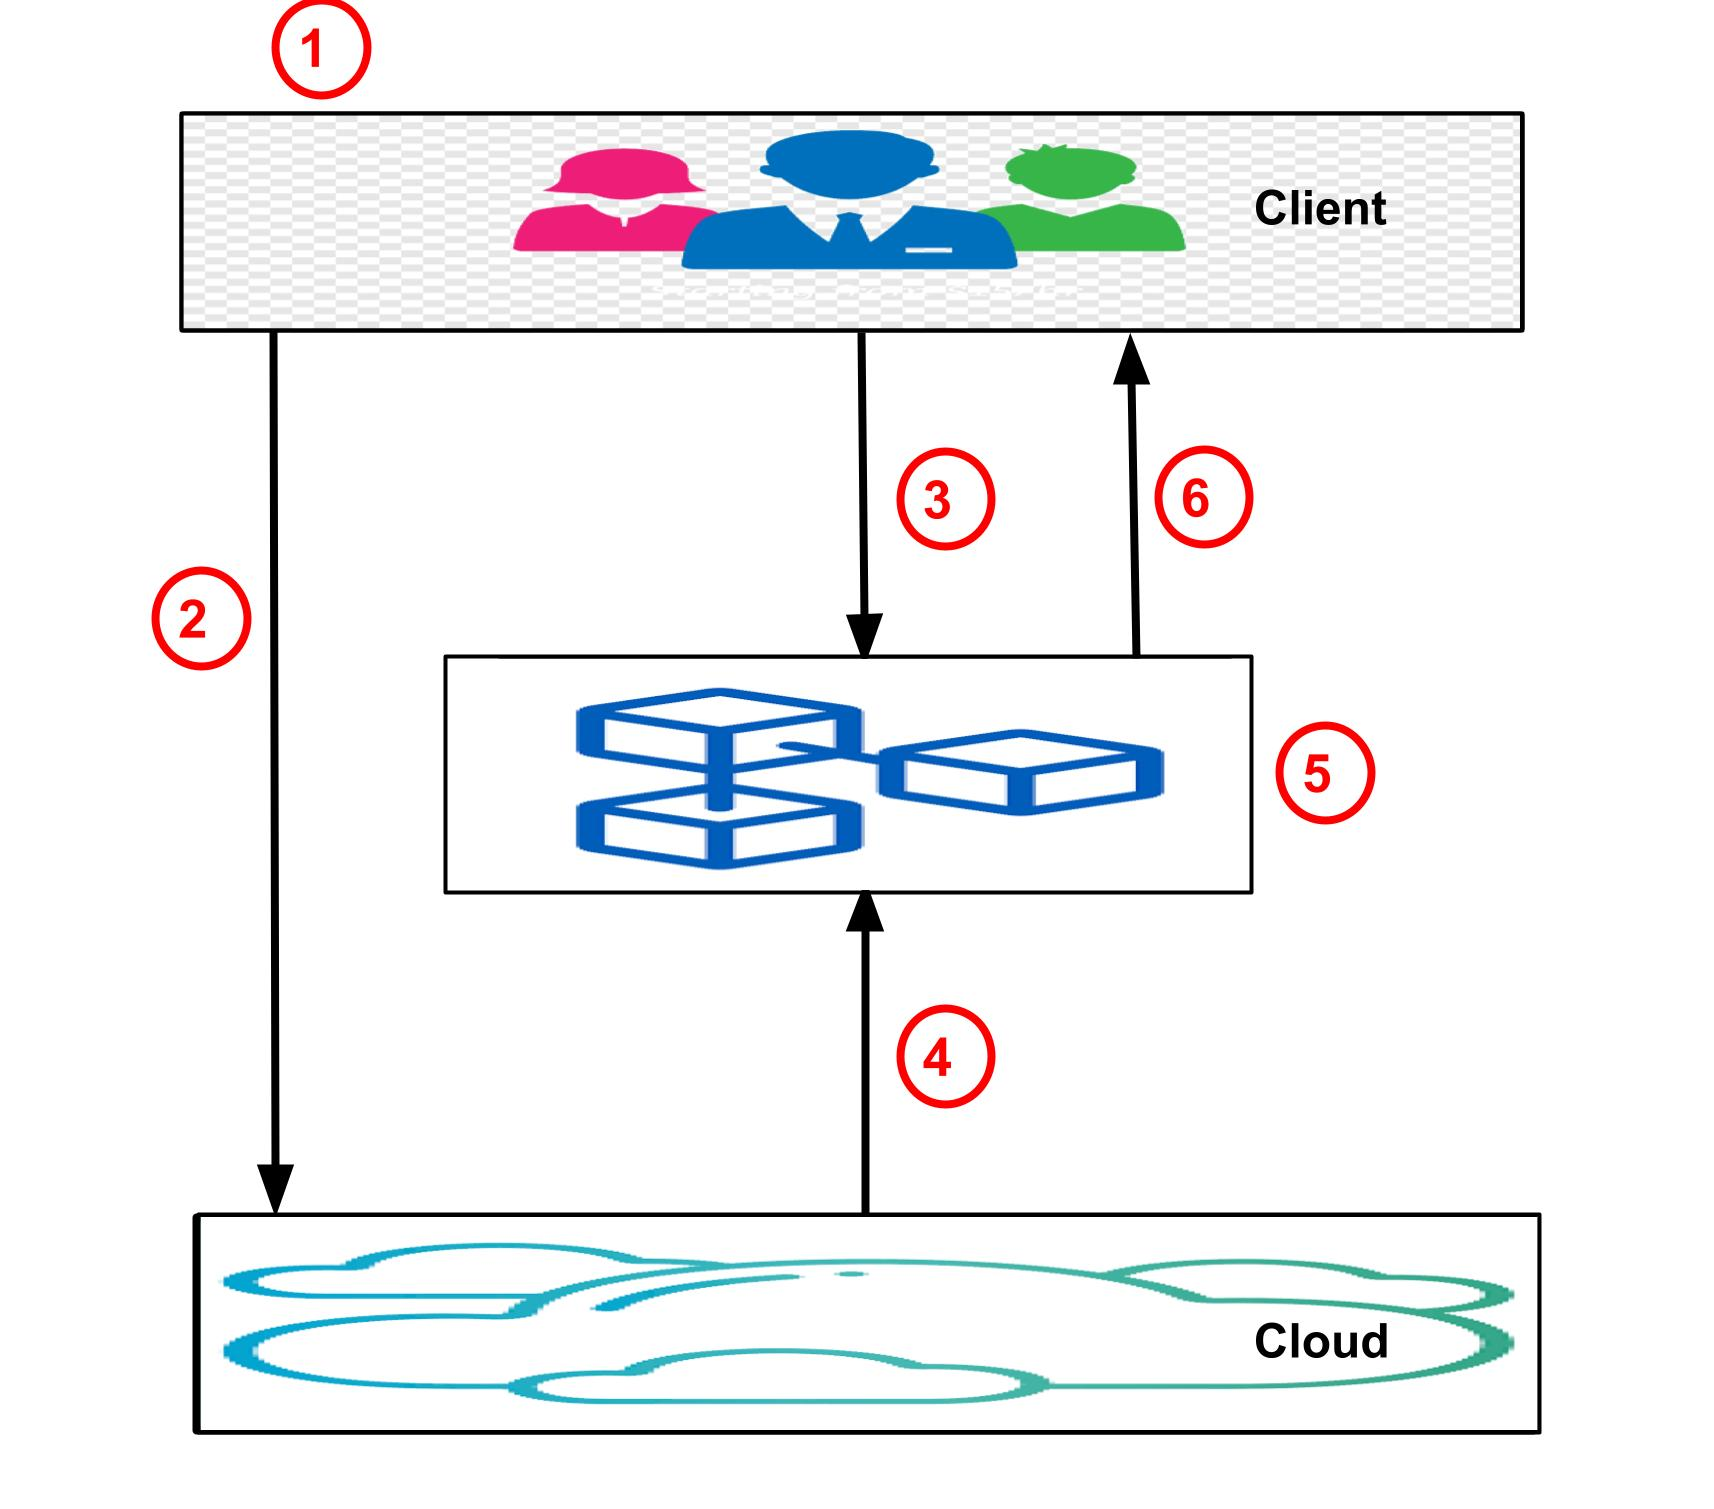
\includegraphics[scale=0.2]{figures/Copy of Untitled drawing (3).jpg}
    \caption{The process of verification phase}
 
\end{figure}

1) Generate audit query chal.

2) Send chal.

3) Send chal.

4) Send the relevant hashes, signatures, random queries and auxiliary information.

5) Calculate Root’ and compare whether Root’ and Root are equal.
 
6)Verify the result.

\subsection{Security Analysis}

\textbf{Anti-forgery attack}
Cloud forges data information with the intention of deceiving the blockchain and the client to pass verification.
It causes a change in the root of the Merkle tree generated by its signatures.
Original hash tree root value Root stored on the blockchain will not change.Then it will be impossible to pass the verification.

\textbf{Anti-fraud attack}
The client uploads corrupt data blocks and then claims that the data is intact to trick the cloud into getting compensation.
To avoid this, the cloud performs a verification before storing the client's data. Cloud verifies the integrity of the data to the blockchan.

\textbf{Data Privacy}
The specific information in the data file is not visible to the cloud. what the cloud has is the encrypted data file and its signature.
The signature set hides the data information well using hash functions, system parameters, client public keys, etc.

\textbf{Detactability}
Data stored in the cloud, if corrupted, can be detected with a probability of no less than 1 −((n-x)/n)m.
This probability is equivalent to that in 1,000,000 data blocks, if 1 percent of the data blocks are damaged, the verifier only selects 300 data blocks, and the detection rate reaches 95 percent. In one challenge, the confidence level CL = P >= 1 −((n-x)/n)m.






